%!TEX root = report.tex
When running the perceptron we obtained several interesting results. We have ran the perceptron for 25, 50 and 100 neurons with $n_d = 200$ and $n_{max} = 500$. Using these parameters, we determined the fraction of successes, or cases where the dataset is linearly separable, over the number of runs. The observed values are plotted against the expected fraction of linearly separable datasets.
\begingroup
    \centering
    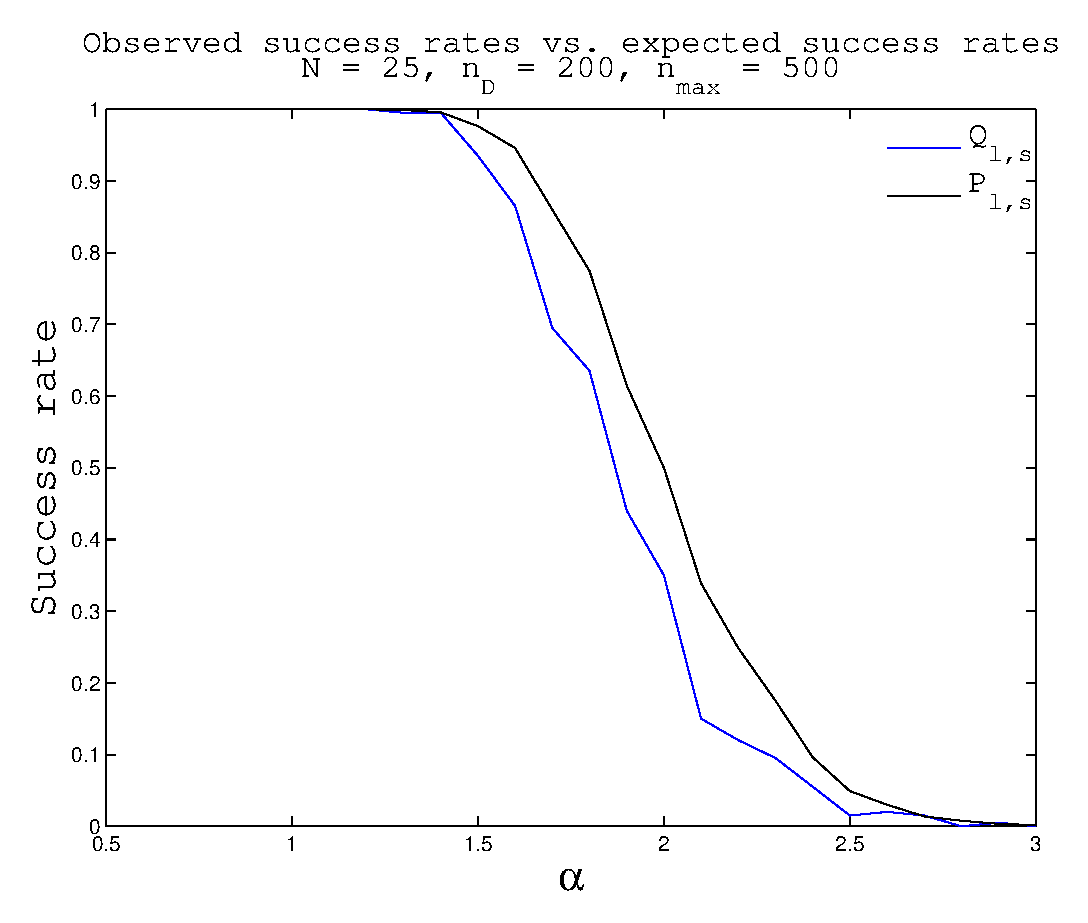
\includegraphics[width=\linewidth]{success_rate_N_25_nd_200_nmax_500.eps}
    \captionof{figure}{Observed success rate versus expected success rate for 25 neurons\newline}\label{fig:25neurons}
\endgroup


Figure~\ref{fig:25neurons} plots the observed linearly separable fraction versus the expected fraction for 25 neurons. It is clear that as $\alpha$ increases the fraction of linearly separable function decreases. This is a first indication that there exists a critical value $\alpha_{c}$ above which there exists no linearly separable dataset.
\begingroup
    \centering
    \includegraphics[width=\linewidth]{success_rate_N_50_nd_200_nmax_500.eps}
    \captionof{figure}{Observed success rate versus expected success rate for 50 neurons\newline}\label{fig:50neurons}
\endgroup


\begingroup
    \centering
    \includegraphics[width=\linewidth]{success_rate_N_100_nd_200_nmax_500.eps}
    \captionof{figure}{Observed success rate versus expected success rate for 100 neurons\newline}\label{fig:100neurons}
\endgroup

